% !TEX root = saveliev_physics_general_course_2.tex
%!TEX TS-program = pdflatex
%!TEX encoding = UTF-8 Unicode


\chapter{ELECTRIC FIELD IN DIELECTRICS}\label{chap:2}

\section{Polar and Non-Polar Molecules}\label{sec:2_1}

Dielectrics (or insulators) are defined as substances not capable of conducting an electric current. Ideal insulators do not exist in nature. All substances, even if to a negligible extent, conduct an electric current. But substances called conductors conduct a current from \num{e15} to \num{e20} times better than substances called dielectrics.

If a dielectric is introduced into an electric field, then the field and the dielectric itself undergo appreciable changes. To understand why this happens, we must take into account that atoms and molecules contain positively charged nuclei and negatively charged electrons.

A molecule is a system with a total charge of zero. The linear dimensions of this system are very small, of the order of a few angstroms (the angstrom---\si{\angstrom}---is a unit of length equal to \SI{e-10}{\metre} that is very convenient in atomic physics). We established in \sect{1_10} that the field set up by such a system is determined by the magnitude and orientation of the dipole electric moment
\begin{equation}\label{eq:2_1}
    \vec{p} = \sum_i q_i \vec{r}_i
\end{equation}

\noindent
(summation is performed both over the electrons and over the nuclei). True, the electrons in a molecule are in motion, so that this moment constantly changes. The velocities of the electrons are so high, however, that the mean value of the moment \eqref{eq:2_1} is detected in practice. For this reason in the following by the dipole moment of a molecule, we shall mean the quantity
\begin{equation}\label{eq:2_2}
    \vec{p} = \sum_i q_i \average{\vec{r}_i}
\end{equation}

\noindent
(for nuclei, $\vec{r}_i$ is simply taken as $\average{\vec{r}_i}$ in this sum). In other words, we shall consider that the electrons are at rest relative to the nuclei at certain points obtained by averaging the positions of the electrons in time.

The behaviour of a molecule in an external electric field is also determined by its dipole moment. We can verify this by calculating the potential energy of a molecule in an external electric field. Selecting the origin of coordinates inside the molecule and taking advantage of the smallness of $\average{\vec{r}_i}$, let us write the potential at the point where the $i$-th charge is in the form
\begin{equation*}
    \varphi_i = \varphi + \gradop{\varphi} \ccdot \average{\vec{r}_i}
\end{equation*}

\noindent
where $\varphi$ is the potential at the origin of coordinates [see \eqn{1_69}]. Hence,
\begin{equation*}
    \ab{W}{p} = \sum_i q_i \varphi_i = \sum_i q_i \parenthesis{\varphi + \gradop{\varphi} \ccdot \average{\vec{r}_i}} = \varphi \sum_i q_i + \gradop{\varphi} \sum_i q_i \average{\vec{r}_i}.
\end{equation*}

\noindent
Taking into account that $\sum_i q_i=0$ and substituting $-\vec{E}$ for $\gradop{\varphi}$, we get
\begin{equation*}
    \ab{W}{p} = -\vec{E} \sum_i q_i \average{\vec{r}_i} = -\vecdot{p}{E} = -p E \cos\alpha.
\end{equation*}

\noindent
Differentiating this expression with respect to $\alpha$, we get \eqn{1_57} for the rotational moment; differentiating with respect to $x$, we arrive at the force \eqref{eq:1_62}.

Thus, a molecule is equivalent to a dipole both with respect to the field it sets up and with respect to the forces it experiences in an external field. The positive charge of this dipole equals the total charge of the nuclei and is at the ``centre of gravity'' of the positive charges; the negative charge equals the total charge of the electrons and is at the ``centre of gravity'' of the negative charges.

In symmetrical molecules (such as \ce{H2},\ce{O2}, \ce{N2}), the centres of gravity of the positive and negative charges coincide in the absence of an external electric field. Such molecules have no intrinsic dipole moment and are called \textbf{non-polar}. In asymmetrical molecules (such
as \ce{CO}, \ce{NH}, \ce{HCl}), the centres of gravity of the charges of opposite signs are displaced relative to each other. In this case, the molecules have an intrinsic dipole moment and are called \textbf{polar}.

Under the action of an external electric field, the charges in a non-polar molecule become displaced relative to one another, the positive ones in the direction of the field, the negative ones against the field. As a result, the molecule acquires a dipole moment whose magnitude, as shown by experiments, is proportional to the field strength (intensity). In the rationalized system, the constant of proportionality is written in the form $\varepsilon_0\beta$, where $\varepsilon_0$ is the electric constant, and $\beta$ is a quantity called the \textbf{polarizability of a molecule}. Since the directions of $\vec{p}$ and $\vec{E}$ coincide, we can write that
\begin{equation}\label{eq:2_3}
    \vec{p} = \beta \varepsilon_0 \vec{E}.
\end{equation}

\noindent
The dipole moment has a dimension of [$q$]L. By \eqn{1_15}, the dimension of $\varepsilon_0\vec{E}$ is [$q$]L$^{-2}$. Hence, the polarizability of a molecule $\beta$ has the dimension L$^3$.

The process of polarization of a non-polar molecule proceeds as if the positive and negative charges of the molecule were bound to one another by elastic forces. A non-polar molecule is, therefore said, to behave in an external field like an elastic dipole.

The action of an external field on a polar molecule consists mainly in tending to rotate the molecule so that its dipole moment is arranged in the direction of the field. An external field does not virtually affect the magnitude of a dipole moment. Consequently, a polar molecule behaves in an external field like a rigid dipole.

\section{Polarization of Dielectrics}\label{sec:2_2}

In the absence of an external electric field, the dipole moments of the molecules of a dielectric usually either equal zero (non-polar molecules) or are distributed in space by directions chaotically (polar molecules). In both cases, the total dipole moment of a dielectric equals zero\footnote{In \sect{2_9}, we shall acquaint ourselves with substances that can have a dipole moment in the absence of an external field.}.

A dielectric becomes polarized under the action of an external field. This signifies that the resultant dipole moment of the dielectric becomes other than zero. It is quite natural to take the dipole moment of a unit volume as the quantity characterizing the degree of polarization. If the field or the dielectric (or both) are not homogeneous, the degrees of polarization at different points of the dielectric will differ. To characterize the polarization at a given point, we must separate an infinitely small (physically) volume $\Delta{V}$ containing this point, find the sum $\sum_{\Delta{V}}\vec{p}$ of the moments of the molecules confined in this volume, and take the ratio
\begin{equation}\label{eq:2_4}
    \vec{P} = \frac{\displaystyle\sum_{\Delta{V}}\vec{p}}{\Delta{V}}.
\end{equation}

\noindent
The vector quantity $\vec{P}$ defined by \eqn{2_4} is called the \textbf{polarization of a dielectric}.

The dipole moment $\vec{p}$ has the dimension [$q$]L. Consequently, the dimension of $\vec{P}$ is [$q$]L$^{-2}$, \ie, it coincides with the dimension of $\varepsilon_0\vec{E}$ [see \eqn{1_15}].

The polarization of isotropic dielectrics of any kind is associated with the field strength at the same point by the simple relation
\begin{equation}\label{eq:2_5}
    \vec{P} = \chi \varepsilon_0 \vec{E}
\end{equation}

\noindent
where $\chi$ is a quantity independent of $\vec{E}$ called the \textbf{electric susceptibility of a dielectric}\footnote{In anisotropic dielectrics, the directions of $\vec{P}$ and $\vec{E}$, generally speaking,
do not coincide. In this case, the relation between $\vec{P}$ and $\vec{E}$ is described by the equations
\begin{align*}
    P_x &= \varepsilon\parenthesis{\chi_{xx}E_x + \chi_{xy}E_y+\chi_{xz}E_z},\\
    P_y &= \varepsilon\parenthesis{\chi_{yx}E_x + \chi_{yy}E_y+\chi_{yz}E_z},\\
    P_z &= \varepsilon\parenthesis{\chi_{zx}E_x + \chi_{zy}E_y+\chi_{zz}E_z}.
\end{align*}

\noindent
The combination of the nine quantities $\chi_{ij}$ forms a symmetrical tensor of rank two called the \textbf{tensor of the dielectric susceptibility} [compare with Eqs. (5.30)
of Vol. I). This tensor characterizes the electrical properties of an anisotropic dielectric.}. It was indicated above that the dimensions of $\vec{P}$ and $\varepsilon_0\vec{E}$ are identical. Hence, $\chi$ is a dimensionless quantity.

In the Gaussian system of units, \eqn{2_5} has the form
\begin{equation}\label{eq:2_6}
    \vec{P} = \chi \vec{E}.
\end{equation}

For dielectrics built of non-polar molecules, \eqn{2_5} issues from the following simple considerations. The volume $\Delta{V}$ contains a number of molecules equal to $n\Delta{V}$, where $n$ is the number of molecules per unit volume. Each of the moments $\vec{p}$ is determined in this case by \eqn{2_3}. Hence,
\begin{equation*}
    \sum{\Delta{V}} \vec{p} = n \Delta{V} \beta \varepsilon_0 \vec{E}.
\end{equation*}

\noindent
Dividing this expression by $\Delta{V}$, we get the polarization $\vec{P}=n\beta\varepsilon_0\vec{E}$. Finally, introducing the symbol $\chi=n\beta$, we arrive at \eqn{2_5}.

For dielectrics built of polar molecules, the orienting action of the external field is counteracted by the thermal motion of the molecules tending to scatter their dipole moments in all directions. As a result, a certain preferred orientation of the dipole moments of the molecules sets in in the direction of the field. The relevant statistical calculations, which agree with experimental data, show that the polarization is proportional to the field strength, \ie, leads to \eqn{2_5}. The electric susceptibility of such dielectrics varies inversely with the absolute temperature.

In ionic crystals, the separate molecules lose their individuality. An entire crystal is, as it were, a single giant molecule. The lattice of an ionic crystal can be considered as two lattices inserted into each other, one of which is formed by the positive, and the other by the negative ions. When an external field acts on the crystal ions, both lattices are displaced relative to each other, which leads to polarization of the dielectric. The polarization in this case too is associated with the field strength by \eqn{2_5}. We must note that the linear relation between $\vec{E}$ and $\vec{P}$ described by \eqn{2_5} may be applied only to not too strong fields [a similar remark relates to \eqn{2_3}].

\section{The Field Inside a Dielectric}\label{sec:2_3}

The charges in the molecules of a dielectric are called \textbf{bound}. The action of a field can only cause bound charges to be displaced slightly from their equilibrium positions; they cannot leave the molecule containing them.

Following the example of L. Landau and E. Lifshitz\footnote{See L. D. Landau and E. M. Lifshitz. Elektrodinamika sploshnykh sred (Electrodynamics of Continuous Media). Moscow, Gostekhizdat (1957), p. 57.}, we shall call charges that, although they are within the boundaries of a dielectric, are not inside its molecules, and also charges outside a dielectric, extraneous ones\footnote{It is customary practice to call such charges \textbf{free}. This name is extremely unsuccessful, however, because in a number of cases extraneous charges are not at all free.}.

The field in a dielectric is the superposition of the field $\ab{\vec{E}}{extr}$ produced by the extraneous charges, and the field $\ab{\vec{E}}{bound}$ of the bound charges. The resultant field is called \textbf{microscopic} (or \textbf{true}):
\begin{equation}\label{eq:2_7}
    \ab{\vec{E}}{micro} = \ab{\vec{E}}{extr} + \ab{\vec{E}}{bound}.
\end{equation}

The microscopic field changes greatly within the limits of the intermolecular distances. Owing to the motion of the bound charges, the field $\ab{\vec{E}}{micro}$ also changes with time. These changes are not detected in a macroscopic-consideration. Therefore, a field is characterized by the quantity \eqref{eq:2_7} averaged over an infinitely small (physically) volume, \ie,
\begin{equation*}
    \vec{E} = \average{\ab{\vec{E}}{micro}} = \average{\ab{\vec{E}}{extr}} + \average{\ab{\vec{E}}{bound}}.
\end{equation*}

In the following, we shall designate the averaged field of the extraneous charges by $\vec{E}_0$, and the averaged field of the bound charges by $\vec{E}'$. Accordingly, we shall define a macroscopic field as the quantity
\begin{equation}\label{eq:2_8}
    \vec{E} = \vec{E}_0 + \vec{E}'.
\end{equation}

The polarization $\vec{P}$ is a macroscopic quantity. Therefore, $\vec{E}$ in \eqn{2_5} should be understood as the strength determined by \eqn{2_8}.

In the absence of dielectrics (\ie, in a ``vacuum''), the macroscopic field is
\begin{equation*}
    \vec{E} = \vec{E}_0 = \average{\ab{\vec{E}}{extr}}.
\end{equation*}

\noindent
It is exactly this quantity that is understood to be $\vec{E}$ in \eqn{1_117}.

If the extraneous charges are stationary, the field determined by \eqn{2_8} has the same properties as an electrostatic field in a vacuum. In particular, it can be characterized with the aid of the potential $\varphi$ related to the field strength \eqref{eq:2_8} by Eqs. \eqref{eq:1_41} and \eqref{eq:1_45}.

\section{Space and Surface Bound Charges}\label{sec:2_4}

When a dielectric is not polarized, the volume density $\rho'$ and the surface density $\sigma'$ of the bound charges equal zero. Polarization causes the surface density, and in some cases also the volume density of the bound charges to become different from zero.

Figure \ref{fig:2_1} shows schematically a polarized dielectric with nonpolar (a) and polar (b) molecules. Inspection of the figure shows that the polarization is attended by the appearance of a surplus of bound charges of one sign in the thin surface layer of the dielectric. If the normal component of the field strength $\vec{E}$ for the given section of the surface is other than zero, then under the action of the field, charges of one sign will move away inward, and of the other sign will emerge.

\begin{figure}[t]
	\begin{minipage}[t]{0.64\linewidth}
		\begin{center}
			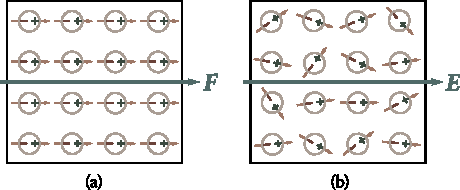
\includegraphics[scale=1]{figures/ch_02/fig_2_1.pdf}
			\caption[]{}
			\label{fig:2_1}
		\end{center}
	\end{minipage}
	\hfill{}%space{-0.05cm}
	\begin{minipage}[t]{0.34\linewidth}
		\begin{center}
			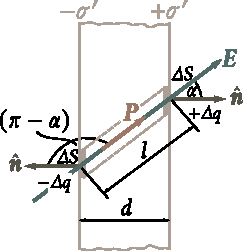
\includegraphics[scale=1]{figures/ch_02/fig_2_2.pdf}
			\caption[]{}
			\label{fig:2_2}
		\end{center}
	\end{minipage}
\vspace{-0.4cm}
\end{figure}

There is a simple relation between the polarization $\vec{P}$ and the surface density of the bound charges $\sigma'$. To find it, let us consider an infinite plane-parallel plate of a homogeneous dielectric placed in a homogeneous electric field (\fig{2_2}). Let us mentally separate an elementary volume in the plate in the form of a very thin cylinder with generatrices parallel to $\vec{E}$ in the dielectric, and with bases of area $\Delta{S}$ coinciding with the surfaces of the plate. The magnitude of this volume is
\begin{equation*}
    \Delta{V} = l \Delta{S} \cos\alpha
\end{equation*}

\noindent
where $l$ is the distance between the bases of the cylinder and $\alpha$ the angle between the vector $\vec{E}$ and an outward normal to the positively charged surface of the dielectric.

The volume $\Delta{V}$ has a dipole electric moment of the magnitude
\begin{equation*}
    P\Delta{V} = Pl\Delta{S}\cos\alpha
\end{equation*}

\noindent
($P$ is the magnitude of the polarization).

From the macroscopic viewpoint, the volume being considered is equivalent to a dipole formed by the $+\sigma'\Delta{S}$ and $-\sigma'\Delta{S}$ with a spacing of $l$. Therefore, its electric moment can be written in the form $\sigma'\Delta{S}l$. Equating the two expressions for the electric moment, we get
\begin{equation*}
    Pl\Delta{S}\cos\alpha = \sigma'\Delta{S}l.
\end{equation*}

\noindent
Hence, we get the required relation between $\sigma'$ and $\vec{P}$:
\begin{equation}\label{eq:2_9}
    \sigma' = P \cos\alpha = \ab{P}{n}
\end{equation}

\noindent
where $\ab{P}{n}$ is the projection of the polarization onto an outward normal to the relevant surface. For the right-hand surface in \fig{2_2}, we have $\ab{P}{n}>0$, accordingly, $\sigma'$ for it is positive; for the left-hand surface $\ab{P}{n}<0$, accordingly, $\sigma'$ for it is negative.

Expressing $\vec{P}$ through $\chi$ and $\vec{E}$ by means of \eqn{2_5}, we arrive at the formula
\begin{equation}\label{eq:2_10}
    \sigma' = \chi \varepsilon_0 \ab{E}{n}
\end{equation}

\noindent
where $\ab{E}{n}$ is the normal component of the field strength inside the dielectric. According to \eqn{2_10}, at the places where the field lines emerge from the dielectric ($\ab{E}{n}>0$), positive bound charges come up to the surface, while where the field lines enter the dielectric ($\ab{E}{n}<0$), negative surface charges appear.

Equations \eqref{eq:2_9} and \eqref{eq:2_10} also hold in the most general case when an inhomogeneous dielectric of an arbitrary shape is in an inhomogeneous electric field. By $\ab{P}{n}$ and $\ab{E}{n}$ in this case, we must understand the normal component of the relevant vector taken in direct proximity to the surface element for which $\sigma'$ is being determined.

Now let us turn to finding the volume density of the bound charges appearing inside an inhomogeneous dielectric. Let us consider an imaginary small area $\Delta{S}$ (\fig{2_3}) in an inhomogeneous isotropic dielectric with non-polar molecules.
Assume that a unit volume of the dielectric has $n$ identical particles with a charge of $+e$ and $n$ identical particles with a charge of $-e$. In close proximity to area $\Delta{S}$, the electric field and the dielectric can be considered homogeneous.
Therefore, when the field is switched on, all the positive charges near $\Delta{S}$ will be displaced over the same distance $l_1$ in the direction of $\vec{E}$, and all the negative charges will be displaced in the opposite direction over the same distance $l_2$ (see \fig{2_3}).
A certain number of charges of one sign (positive if $\alpha<n/2$ and negative if $\alpha>n/2$) will pass through area $\Delta{S}$ in the direction of a normal to it, and a certain number of charges of the opposite sign (negative if $\alpha<n/2$ and positive if $\alpha<n/2$) in the direction opposite to $\hatvec{n}$.
Area $\Delta{S}$ will be intersected by all the charges $+e$ that were at a distance of not over $l_1\cos\alpha$ from it before the field was switched on, \ie, by all the $+e$'s in an oblique cylinder of volume $l_1\Delta{S}\cos\alpha$. The number of these charges is $nl_1\Delta{S}\cos\alpha$, while the charge they carry in the direction of a normal to the area is $enl_1\Delta{S}\cos\alpha$ (when $\alpha>\pi/2$, the charge carried in the direction of the normal as a result of displacement of the charges $+e$ will be negative).
Similarly, area $\Delta{S}$ will be intersected by all the charges $-e$ in the volume $l_2\Delta{S}\cos\alpha$. These charges will carry a charge of $enl_2\Delta{S}\cos\alpha$ in the direction of a normal to the area (inspection of \fig{2_3} shows that when $\alpha<\pi/2$, the charges $-e$ will carry the charge $-enl_2\Delta{S}\cos\alpha$ through $\Delta{S}$ in the direction opposite to $\hatvec{n}$, which is equivalent to carrying the charge $enl_2\Delta{S}\cos\alpha$ in the direction of $\hatvec{n}$).

\begin{figure}[t]
	\begin{center}
		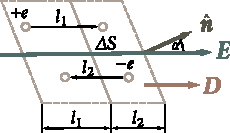
\includegraphics[scale=1.1]{figures/ch_02/fig_2_3.pdf}
		\caption[]{}
		\label{fig:2_3}
	\end{center}
	\vspace{-0.8cm}
\end{figure}

Thus, when the field is switched on, the charge
\begin{equation*}
    \Delta{q}' = enl_1\Delta{S}\cos\alpha + enl_2\Delta{S}\cos\alpha = en (l_1+l_2) \Delta{S} \cos\alpha
\end{equation*}

\noindent
is carried through area $\Delta{S}$ in the direction of a normal to it. The sum $l_1+l_2$ is the distance $l$ over which the positive and negative bound charges are  displaced toward one another in the dielectric. As a result of this displacement, each pair of charges acquires the dipole moment $p=el=e(l_1+l_2)$. The number of such pairs in a unit volume is $n$. Consequently, the product $e(l_1+l_2)n=eln=p$ gives the magnitude of the polarization $P$. Thus, the charge passing through area $\Delta{S}$ in the direction of a normal to it when the field is switched on is [see \eqn{2_9}]
\begin{equation*}
    \Delta{q}' = P \Delta{S} \cos\alpha.
\end{equation*}

Since the dielectric is isotropic, the directions of the vectors $\vec{E}$ and $\vec{P}$ coincide (see \fig{2_3}). Consequently, $\alpha$ is the angle between the vectors $\vec{P}$ and $\hatvec{n}$, and in this connection we can write
\begin{equation*}
    \Delta{q}' = (\vec{P} \ccdot \hatvec{n})\, \Delta{S}.
\end{equation*}

\noindent
Passing over from deltas to differentials, we get
\begin{equation*}
    \deriv{q} = (\vec{P} \ccdot \hatvec{n})\, \deriv{S} = \vec{P} \ccdot \deriv{\vec{S}}.
\end{equation*}

We have found the bound charge $\deriv{q'}$ that passes through elementary area $\deriv{S}$ in the direction of a normal to it when the field is switched on; $\vec{P}$ is the polarization set up under the action of the field at the location of area $\deriv{S}$.

Let us imagine closed surface $S$ inside the dielectric. When the field is switched on, a bound charge $q'$ will intersect this surface and emerge from it. This charge is
\begin{equation*}
    \ab{q'}{em} = \oint_S \deriv{q'} = \oint_S \vec{P} \ccdot \deriv{\vec{S}}
\end{equation*}

\noindent
(we have agreed to take the outward normal to area $\deriv{S}$ for closed surfaces). As a result, a surplus bound charge will appear in the volume enclosed by surface $S$. Its value is
\begin{equation}\label{eq:2_11}
    \ab{q'}{sur} = - \ab{q'}{em} = - \oint_S \vec{P} \ccdot \deriv{\vec{S}} = - \ab{\Phi}{P}
\end{equation}

\noindent
($\ab{\Phi}{P}$ is the flux of the vector $\vec{P}$ through surface $S$).

Introducing the volume density of the bound charges $\rho'$, we can write
\begin{equation*}
    \ab{q'}{sur} = \int_V \rho'\, \deriv{V}
\end{equation*}

\noindent
(the integral is taken over the volume enclosed by surface $S$). We thus arrive at the formula
\begin{equation*}
    \int_V \rho'\, \deriv{V} = - \oint_S \vec{P} \ccdot \deriv{\vec{S}}.
\end{equation*}

\noindent
Let us transform the surface integral according to the Ostrogradsky-Gauss theorem [see \eqn{1_108}). The result is
\begin{equation*}
    \int_V \rho'\, \deriv{V} = - \int_V \divop{\vec{P}}\, \deriv{V}.
\end{equation*}

\noindent
This equation must be observed for any arbitrarily chosen volume $V$. This is possible only if the following equation is observed at every point of the dielectric:
\begin{equation}\label{eq:2_12}
    \rho' = - \divop{\vec{P}}.
\end{equation}

\noindent
Consequently, the density of bound charges equals the divergence of the polarization $\vec{P}$ taken with the opposite sign.

We obtained \eqn{2_12} when considering a dielectric with non-polar molecules. This equation also holds, however, for dielectrics with polar molecules.

\begin{figure}[t]
	\begin{center}
		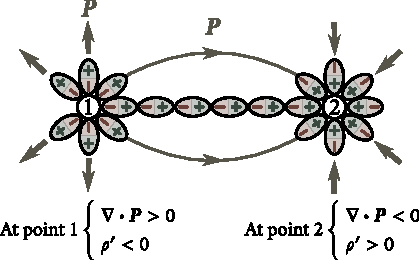
\includegraphics[scale=1]{figures/ch_02/fig_2_4.pdf}
		\caption[]{}
		\label{fig:2_4}
	\end{center}
	\vspace{-0.8cm}
\end{figure}

Equation \eqref{eq:2_12} can be given a graphical interpretation. Points with a positive $\divop{\vec{P}}$ are sources of the field of the vector $\vec{P}$, and the lines of $\vec{P}$ diverge from them (\fig{2_4}). Points with a negative $\divop{\vec{P}}$ are sinks of the field of the vector $\vec{P}$, and the lines of $\vec{P}$ converge at them.
In polarization of the dielectric, the positive bound charges are displaced in the direction of the vector $\vec{P}$, \ie, in the direction of the lines $\vec{P}$; the negative bound charges are displaced in the opposite direction (in the figure the bound charges belonging to separate molecules are encircled by ovals). As a result, a surplus of negative bound charges is formed at places with a positive $\divop{\vec{P}}$, and a surplus of positive bound charges at places with a negative $\divop{\vec{P}}$.

Bound charges differ from extraneous ones only in that they cannot leave the confines of the molecules which they are in. Otherwise, they have the same properties as all other charges. In particular, they are sources of an electric field. Therefore, when the density of the bound charges $\rho'$ differs from zero, \eqn{1_117} must be written in the form
\begin{equation}\label{eq:2_13}
    \divop{\vec{E}} = \frac{1}{\varepsilon_0} \parenthesis{\rho + \rho'}.
\end{equation}

\noindent
Here $\rho$ is the density of the extraneous charges.

Let us introduce \eqn{2_5} for $\vec{P}$ into \eqn{2_12} and use \eqn{1_103}. The result is
\begin{equation*}
    \rho' = - \divop{(\chi\varepsilon_0\vec{E})} = - \varepsilon_0 \divop{(\chi\vec{E})} = - \varepsilon_0 [\vec{E}\ccdot\gradop{\chi} + \chi \divop{\vec{E}}].
\end{equation*}

\noindent
Substituting for $\divop{\vec{E}}$ its value from \eqn{2_13}, we arrive at the equation
\begin{equation*}
    \rho' = - \varepsilon_0 (\vec{E}\ccdot\gradop{\chi}) - \chi\rho - \chi\rho'.
\end{equation*}

\noindent
Hence,
\begin{equation}\label{eq:2_14}
    \rho' = - \parenthesis{\frac{1}{1+\chi}} [\varepsilon_0 (\vec{E}\ccdot\gradop{\chi}) + \chi\rho].
\end{equation}

We can see from \eqn{2_14} that the volume density of bound charges can differ from zero in two cases: (1) if a dielectric is not homogeneous ($\gradop{\chi}\neq 0$), and (2) if at a given place in a dielectric the density of the extraneous charges is other than zero ($\rho\neq 0$).

When there are no extraneous charges in a dielectric, the volume density of the bound charges is
\begin{equation}\label{eq:2_15}
    \rho' = - \parenthesis{\frac{\varepsilon_0}{1+\chi}} (\vec{E}\ccdot\gradop{\chi}).
\end{equation}

\section{Electric Displacement Vector}\label{sec:2_5}

We noted in the preceding section that not only extraneous, but also bound charges are sources of a field. Accordingly,
\begin{equation}\label{eq:2_16}
    \divop{\vec{E}} = \frac{1}{\varepsilon_0} \parenthesis{\rho + \rho'}
\end{equation}

\noindent
[see \eqn{2_13}].

Equation \eqref{eq:2_16} is of virtually no use for finding the vector $\vec{E}$ because it expresses the properties of the unknown quantity $\vec{E}$ through bound charges, which in turn are determined by the unknown quantity $\vec{E}$ [see Eqs. \eqref{eq:2_10} and \eqref{eq:2_14}].

Calculation of the fields is often simplified if we introduce an auxiliary quantity whose sources are only extraneous charges $\rho$. To establish what this quantity looks like, let us introduce \eqn{2_12} for $\rho'$ into \eqn{2_16}:
\begin{equation*}
    \divop{\vec{E}} = \frac{1}{\varepsilon_0} (\rho - \divop{\vec{P}})
\end{equation*}

\noindent
whence it follows that
\begin{equation}\label{eq:2_17}
    \divop{(\varepsilon_0\vec{E} + \vec{P})} = \rho
\end{equation}

\noindent
(we have put $\varepsilon_0$ inside the del symbol). The expression in parentheses in \eqn{2_17} is the required quantity. It is designated by the symbol $\vec{D}$ and is called the electric displacement (or electric induction).

Thus, the \textbf{electric displacement} is a quantity determined by the relation
\begin{equation}\label{eq:2_18}
    \vec{D} = \varepsilon_0\vec{E} + \vec{P}.
\end{equation}

\noindent
Inserting \eqn{2_5} for $\vec{P}$, we get
\begin{equation}\label{eq:2_19}
    \vec{D} = \varepsilon_0\vec{E} + \chi\varepsilon_0\vec{E} = \varepsilon_0 (1+\chi) \vec{E}.
\end{equation}

The dimensionless quantity
\begin{equation}\label{eq:2_20}
    \varepsilon = 1 + \chi
\end{equation}

\noindent
is called the \textbf{relative permittivity} or simply the \textbf{permittivity} of a medium\footnote{The so-called absolute permittivity of a medium $\ab{\varepsilon}{a}=\varepsilon_0\varepsilon$ is introduced in electrical engineering. This quantity is deprived of a physical meaning, however, and we shall not use it.}. Thus, \eqn{2_19} can be written in the form
\begin{equation}\label{eq:2_21}
    \vec{D} = \varepsilon_0 \varepsilon \vec{E}.
\end{equation}

\noindent
According to \eqn{2_21}, the vector $\vec{D}$ is proportional to the vector $\vec{E}$. We remind our reader that we are dealing with isotropic dielectrics. In anisotropic dielectrics, the vectors $\vec{E}$ and $\vec{D}$, generally speaking, are not collinear.

In accordance with Eqs. \eqn{1_15} and \eqn{2_21}, the electric displacement of the field of a point charge in a vacuum is
\begin{equation}\label{eq:2_22}
    \vec{D} = \frac{1}{4\pi} \frac{q}{r^2} \vecuni{r}.
\end{equation}

The unit of electric displacement is the coulomb per square
metre (\si{\coulomb\per\metre\squared}).

Equation \eqref{eq:2_17} can be written as
\begin{equation}\label{eq:2_23}
    \divop{\vec{D}} = \rho.
\end{equation}

\noindent
Integration of this equation over the arbitrary volume $V$ yields
\begin{equation*}
    \int_V \divop{\vec{D}}\, \deriv{V} = \int_V \rho\, \deriv{V}.
\end{equation*}

\noindent
Let us transform the left-hand side according to the Ostrogradsky-Gauss theorem [see \eqn{1_108}]:
\begin{equation}\label{eq:2_24}
    \oint_S \vec{D} \ccdot \deriv{\vec{S}} = \int_V \rho\, \deriv{V}.
\end{equation}

\noindent
The quantity on the left-hand side is $\Phi_D$---the flux of the vector $\vec{D}$ through closed surface $S$, while that on the right-hand side is the sum of the extraneous charges $\sum_iq_i$ enclosed by this surface. Hence, \eqn{2_24} can be written in the form
\begin{equation}\label{eq:2_25}
    \Phi_D = \sum_i q_i.
\end{equation}

\noindent
Equations \eqref{eq:2_24} and \eqref{eq:2_25} express Gauss's theorem for the vector $\vec{D}$: \textit{the flux of the electric displacement through a closed surface equals the algebraic sum of the extraneous charges enclosed by this surface}.

In a vacuum, $\vec{P}=0$, so that the quantity $\vec{D}$ determined by \eqn{2_18} transforms into $\varepsilon_0\vec{E}$, and Eqs. \eqref{eq:2_24} and \eqref{eq:2_25} transform into Eqs. \eqref{eq:1_114} and \eqref{eq:1_116}.

The unit of the flux of the electric displacement vector is the coulomb. By \eqn{2_25}, a charge of \SI{1}{\coulomb} sets up a displacement flux of \SI{1}{\coulomb} through the surface surrounding it.

The field of the vector $\vec{D}$ can be depicted with the aid of electric displacement lines (we shall call them displacement lines for brevity's sake). Their direction and density are determined in exactly the same way as for the lines of the vector $\vec{E}$ (see \sect{1_5}). The lines of the vector $\vec{E}$ can begin and terminate at both extraneous and bound charges. The sources of the field of the vector $\vec{D}$ are only extraneous charges. Hence, displacement lines can begin or terminate only at extraneous charges. These lines pass without interruption through points at which bound charges are placed.

The electric induction\footnote{The term ``electric displacement'' is not applied to quantity \eqref{eq:2_27}.} in the Gaussian system is determined by the expression
\begin{equation}\label{eq:2_26}
    \vec{D} = \vec{E} + 4\pi\vec{P}.
\end{equation}

\noindent
Substituting for $\vec{P}$ in this equation its value from \eqn{2_6}, we get
\begin{equation}\label{eq:2_27}
    \vec{D} = (1 + 4\pi\chi) \vec{E}.
\end{equation}

The quantity
\begin{equation}\label{eq:2_28}
    \varepsilon = 1 + 4\pi\chi.
\end{equation}

\noindent
is called the \textbf{permittivity}. Introducing this quantity into \eqn{2_27} we get
\begin{equation}\label{eq:2_29}
    \vec{D} = \varepsilon \vec{E}.
\end{equation}

In the Gaussian system, the electric induction in a vacuum coincides with the field strength $\vec{E}$. Consequently, the electric induction of the field of a point charge in a vacuum is determined by \eqn{1_16}.

By \eqn{2_22} the electric displacement set up by a charge of \SI{1}{\coulomb} at a distance of \SI{1}{\metre} is
\begin{equation*}
    D = \frac{1}{4\pi}\frac{q}{r^2} = \frac{1}{4\pi\times 1^2} = \frac{1}{4\pi} \si{\coulomb\per\metre\squared}.
\end{equation*}

\noindent
In the Gaussian system, the electric induction in this case is
\begin{equation*}
    D = \frac{q}{r^2} = \frac{\num{3e9}}{\num{e4}} = \SI{3e5}{\cgse{D}}.
\end{equation*}

\noindent
Thus,
\begin{equation*}
    \SI{1}{\coulomb\per\metre\squared} = 4\pi \times  \SI{3e5}{\cgse{D}}.
\end{equation*}

In the Gaussian system, the expressions of Gauss's theorem
have the form
\begin{align}
    \oint_S \vec{D} \ccdot \deriv{\vec{S}} &= 4\pi \int_V \rho\, \deriv{V}\label{eq:2_30}\\
    \Phi_D &= 4\pi \sum_i q_i.\label{eq:2_31}
\end{align}

\noindent
According to \eqn{2_31}, a charge of \SI{1}{\coulomb} sets up a flux of the electric induction vector of $4\pi q=4\pi\times\SI{3e9}{\cgse{\Phi_D}}$. The following relation thus exists between the units of flux of the vector $\vec{D}$:
\begin{equation*}
    \SI{1}{\coulomb} = 4\pi \times \SI{3e9}{\cgse{\Phi_D}}.
\end{equation*}

\section{Examples of Calculating the Field in Dielectrics}\label{sec:2_6}

We shall consider several examples of fields in dielectrics to reveal the meaning of the quantities $\vec{D}$ and $\varepsilon$.

\textbf{Field Inside a Flat Plate.} Let us consider two infinite parallel oppositely charged planes. Let the field they produce in a vacuum be characterized by the strength $\vec{E}_0$ and the displacement $\vec{D}_0=\varepsilon_0\vec{E}_0$. Let us introduce into this field a plate of a homogeneous isotropic dielectric and arrange it as shown in \fig{2_5}. The dielectric becomes polarized under the action of the field, and bound charges of density $\sigma'$ will appear on its surfaces. These charges will set up a homogeneous field inside the plate whose strength by \eqn{1_121} is $E'=\sigma'/\varepsilon_0$. In the given case, $E'=0$ outside the dielectric.

\begin{figure}[t]
	\begin{center}
		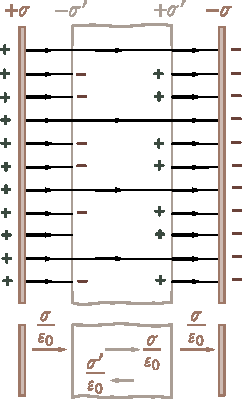
\includegraphics[scale=1]{figures/ch_02/fig_2_5.pdf}
		\caption[]{}
		\label{fig:2_5}
	\end{center}
	\vspace{-0.8cm}
\end{figure}

The field strength $E_0$ is $\sigma/\varepsilon_0$. Both fields are directed toward each other, hence, inside the dielectric we have
\begin{equation}\label{eq:2_32}
    E = E_0 - E' = E_0 - \frac{\sigma'}{\varepsilon_0} = \frac{1}{\varepsilon_0}\parenthesis(\sigma - \sigma').
\end{equation}

\noindent
Outside the dielectric, $E=E_0$.

The polarization of the dielectric is due to field \eqref{eq:2_32}. The latter is perpendicular to the surfaces of the plate. Hence, $\ab{E}{n}=E$, and in accordance with \eqn{2_10}, $\sigma'=\chi\varepsilon_0E$. Using this value in \eqn{2_32}, we get
\begin{equation*}
    E = E_0 - \chi E
\end{equation*}

\noindent
whence
\begin{equation}\label{eq:2_33}
    E = \frac{E_0}{1 + \chi} = \frac{E_0}{\varepsilon}.
\end{equation}

\noindent
Thus, in the given case, the permittivity $\varepsilon$
shows how many times the field in a dielectric weakens.

Multiplying \eqn{2_33} by $\varepsilon_0\varepsilon$, we get the electric displacement inside the plate:
\begin{equation}\label{eq:2_34}
    D = \varepsilon_0 \varepsilon E = \varepsilon_0 E_0 D_0.
\end{equation}

\noindent
Hence, the electric displacement inside the plate coincides with that of the external field $D_0$. Substituting $\sigma/\varepsilon_0$ for $E_0$ in \eqn{2_34}, we find
\begin{equation}\label{eq:2_35}
    D = \sigma.
\end{equation}

To find $\sigma'$, let us express $E$ and $E_0$ in \eqn{2_33} through the charge densities:
\begin{equation*}
    \frac{1}{\varepsilon_0} \parenthesis(\sigma - \sigma') = \frac{\sigma}{\varepsilon_0\varepsilon}
\end{equation*}

\noindent
whence
\begin{equation}\label{eq:2_36}
    \sigma' = \frac{\varepsilon - 1}{\varepsilon} \sigma.
\end{equation}

Figure \ref{fig:2_5} has been drawn assuming that $\varepsilon=3$. Accordingly, the density of the field lines in the dielectric is one-third of that outside the plate. The lines are equally spaced because the field is homogeneous. In the given case, $\sigma'$ can be found without resorting to \eqn{2_36}. Indeed, since the field intensity inside the plate is one-third of that outside it, then of three field lines beginning (or terminating) on
extraneous charges, two must terminate (or begin respectively) on bound charges. It thus follows that the density of the bound charges must be two-thirds that of the extraneous charges.

In the Gaussian system, the field strength $E'$ produced by the bound charges $\sigma'$ is $4\pi\sigma'$. Therefore, \eqn{2_32} becomes
\begin{equation}\label{eq:2_37}
    E = E_0 - E' = E_0 - 4\pi\sigma'.
\end{equation}

\noindent
The surface density $\sigma'$ is associated with the field strength $E$ by the equation $\sigma'=\chi \ab{E}{n}$. We can thus write that
\begin{equation*}
    E = E_0 - 4\pi\chi E
\end{equation*}

\noindent
whence
\begin{equation*}
    E = \frac{E_0}{1 + 4\pi\chi} = \frac{E_0}{\varepsilon}.
\end{equation*}

\noindent
Thus, the permittivity $\varepsilon$, like its counterpart $\varepsilon$ in the SI, shows how many times the field inside a dielectric weakens. Therefore, the values of $\varepsilon$ in the SI and the Gaussian system coincide. Hence, taking into account Eqs. \eqref{eq:2_20} and \eqref{eq:2_28}, we conclude that the susceptibilities in the Gaussian system ($\ab{\chi}{Gs}$) and in the SI ($\ab{\chi}{SI}$) differ from each other by the factor $4\pi$:
\begin{equation}\label{eq:2_38}
    \ab{\chi}{SI} = 4\pi\ab{\chi}{Gs}.
\end{equation}

\textbf{Field Inside a Spherical Layer.} Let us surround a charged sphere of radius $R$ with a concentric spherical layer of a homogeneous isotropic dielectric (\fig{2_6}). The bound charge $q_1'$ distributed with the density $\sigma_1'$ will appear on the internal surface of the layer ($q_1'=4\pi R_1^2\sigma_1'$), and the charge $q_2'$ distributed with the density $\sigma_2'$ will appear on its external surface ($q_2'=4\pi R_2^2\sigma_2'$). The sign of the charge $q_2'$ coincides with that of the charge $q$ of the sphere, while $q_1'$ has the opposite sign.
The charges $q_1'$ and $q_2'$ set up a field at a distance $r$ exceeding $R_1$ and $R_2$, respectively, that coincides with the field of a point charge of the same magnitude [see \eqn{1_124}]. The charges $q_1'$ and $q_2'$ produce no field inside the surfaces over which they are distributed. Hence, the field strength $E'$ inside a dielectric is
\begin{equation*}
    E' = \frac{1}{4\pi\varepsilon_0}\frac{q_1'}{r^2} = \frac{1}{4\pi\varepsilon_0} \frac{4\pi R_1^2\sigma_1'}{r^2} = \frac{1}{\varepsilon_0} \frac{R_1^2 \sigma_1'}{r^2}
\end{equation*}

\noindent
and is opposite in direction to the field strength $E_0$. The resultant field in a dielectric is
\begin{equation}\label{eq:2_39}
    E(r) = E_0 - E' = \frac{1}{4\pi\varepsilon_0} \frac{q}{r^2} - \frac{1}{\varepsilon_0} \frac{R_1^2 \sigma_1'}{r^2}.
\end{equation}

\begin{figure}[t]
	\begin{center}
		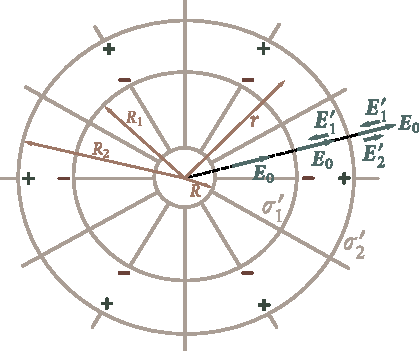
\includegraphics[scale=1.0]{figures/ch_02/fig_2_6.pdf}
		\caption[]{}
		\label{fig:2_6}
	\end{center}
	\vspace{-0.8cm}
\end{figure}

\noindent
It diminishes in proportion to $1/r^2$. We can, therefore, state that
\begin{equation*}
    \frac{E(R_1)}{E(r)} = \frac{r^2}{R_1^2}\quad \Rightarrow\quad E(R_1) = E(r) \frac{r^2}{R_1^2},
\end{equation*}

\noindent
where $E(R_1)$ is the field strength in a dielectric in direct proximity to the internal surface of the layer. It is exactly this strength that determines the quantity $\sigma_1'$:
\begin{equation}\label{eq:2_40}
    \sigma_1' = \chi\varepsilon_0 E(R_1) = \chi\varepsilon_0 E(r) \frac{r^2}{R_1^2}
\end{equation}

\noindent
(at each point of the surface $|\ab{E}{n}|=E$).

Introducing \eqn{2_40} into \eqn{2_39}, we get
\begin{equation*}
    E(r) = \frac{1}{4\pi\varepsilon_0} \frac{q}{r^2} - \frac{1}{\varepsilon_0} \frac{R_1^2 \chi \varepsilon_0 E(r) r^2}{r^2 R_1^2} = E_0(r) - \chi E(r).
\end{equation*}

\noindent
From this equation, we find that inside a dielectric $E=E_0/\varepsilon$, and, consequently, $D=\varepsilon_0E_0$ [compare with Eqs. \eqref{eq:2_33} and \eqref{eq:2_34}].

The field inside a dielectric changes in proportion to $1/r^2$. Therefore, the relation $\sigma_1' :\sigma_2' = R_1 : R_2$ holds. Hence, it follows that $q_1'=q_2'$. Consequently, the fields set up by these charges at distances exceeding $R_2$ mutually destroy each other so that outside the spherical layer $E'=0$ and $E=E_0$.

Assuming that $R_1=R$ and $R_2=\infty$, we arrive at the case of a charged sphere immersed in an infinite homogeneous and isotropic dielectric. The field strength outside such a sphere is
\begin{equation}\label{eq:2_41}
    E = \frac{1}{4\pi\varepsilon_0} \frac{q}{\varepsilon r^2}.
\end{equation}

\noindent
The strength of the field set up in an infinite dielectric by a point charge will be the same.

Both examples considered above are characterized by the fact that the dielectric was homogeneous and isotropic, and the surfaces enclosing it coincided with the equipotential surfaces of the field of extraneous charges. The result we have obtained in these cases is a general one. \textit{If a homogeneous and isotropic dielectric completely fills the volume enclosed by equipotential surfaces of the field of extraneous charges, then the electric displacement vector coincides with the vector of the field strength of the extraneous charges multiplied by $\varepsilon_0$, and, therefore, the field strength inside the dielectric is $1/\varepsilon$ of that of the field strength of the extraneous charges}.

If the above conditions are not observed, the vectors $\vec{D}$ and $\varepsilon_0\vec{E}$ do not coincide. Figure \ref{fig:2_7} shows the field in the plate of a dielectric. The plate is skewed relative to the planes carrying extraneous charges. The vector $\vec{E}'$ is perpendicular to the faces of the plate, therefore, $\vec{E}$ and $\vec{E}_0$ are not collinear. The vector $\vec{D}$ is directed the same as $\vec{E}$, consequently, $\vec{D}$ and $\varepsilon_0\vec{E}_0$ do not coincide in direction. We can show that they also fail to coincide in magnitude.
In the examples considered above owing to the specially selected shape of the dielectric, the field $\vec{E}'$ differed from zero only inside the dielectric. In the general case, $\vec{E}'$ may differ from zero outside the dielectric too. Let us place a rod made of a dielectric into an initially homogeneous field (\fig{2_8}). Owing to polarization, bound charges of opposite signs are formed on the ends of the rod. Their field outside the rod is equivalent to the field of a dipole (the lines of $\vec{E}'$ are dash ones in the figure). It is easy to see that the resultant field $\vec{E}$ near the ends of the rod is greater than the field $\vec{E}_0$.

\begin{figure}[t]
	\begin{minipage}[t]{0.46\linewidth}
		\begin{center}
			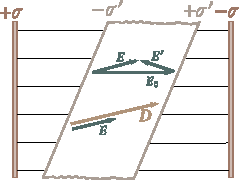
\includegraphics[scale=1.2]{figures/ch_02/fig_2_7.pdf}
			\caption[]{}
			\label{fig:2_7}
		\end{center}
	\end{minipage}
	\hfill{}%space{-0.05cm}
	\begin{minipage}[t]{0.5\linewidth}
		\begin{center}
			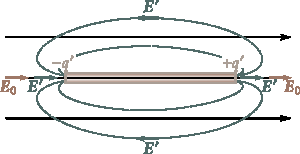
\includegraphics[scale=1.2]{figures/ch_02/fig_2_8.pdf}
			\caption[]{}
			\label{fig:2_8}
		\end{center}
	\end{minipage}
\vspace{-0.4cm}
\end{figure}

\section{Conditions on the Interface Between Two Dielectrics}\label{sec:2_7}

Near the interface between two dielectrics, the vectors $\vec{E}$ and $\vec{D}$ must comply with definite boundary conditions following from the relations \eqref{eq:1_112} and \eqref{eq:2_23}:
\begin{equation*}
    \curlop{\vec{E}} = 0,\quad \divop{\vec{D}} = \rho.
\end{equation*}

Let us consider the interface between two dielectrics with the permittivities $\varepsilon_1$ and $\varepsilon_2$ (\fig{2_9}). We choose an arbitrarily directed $x$-axis on this surface. We take a small rectangular contour of length $a$ and width $b$ that is partly in the first dielectric and partly in the second one. The $x$-axis passes through the middle of the sides $b$.

Assume that a field has been set up in the first dielectric whose strength is $\vec{E}_1$, and in the second one whose strength is $\vec{E}_2$. Since $\curlop{\vec{E}}=0$, the circulation of the vector $\vec{E}$ around the contour we have chosen must equal zero [see \eqn{1_110}]. With small dimensions of the contour and the direction of circumvention shown in \fig{2_9}, the circulation of the vector $\vec{E}$ can be written in the form
\begin{equation}\label{eq:2_42}
    \oint E_l\,\deriv{l} = E_{1,x} a - E_{2,x} a + \average{E_b} 2b
\end{equation}

\noindent
where $\average{E_b}$ is the mean value of $E_l$ on sections of the contour perpendicular to the interface. Equating this expression to zero, we arrive at the equation
\begin{equation*}
    \parenthesis{E_{1,x} - E_{2,x}} a = \average{E_b} 2b.
\end{equation*}

\noindent
In the limit, when the width $b$ of the contour tends to zero, we get
\begin{equation}\label{eq:2_43}
    E_{1,x} = E_{2,x}.
\end{equation}

\noindent
The values of the projections of the vectors $\vec{E}_1$ and $\vec{E}_2$ onto the $x$-axis are taken in direct proximity to the interface between the boundary of the dielectrics.

Equation \eqref{eq:2_43} is obeyed when the $x$-axis is selected arbitrarily. It is only essential that this axis be in the plane of the interface between the dielectrics. Inspection of \eqn{2_43} shows that with such a selection of the $x$-axis when $E_{1,x}=0$, the projection of $E_{2,x}=0$ will also equal zero. This signifies that the vectors $\vec{E}_1$ and $\vec{E}_2$ at two close points taken at opposite sides of the interface are in the same plane as a normal to the interface. Let us represent each of the vectors $\vec{E}_1$ and $\vec{E}_2$ in the form of the sum of the normal and tangential components:
\begin{equation*}
    \vec{E}_1 = \vec{E}_{1,n} + \vec{E}_{1,\tau},\quad \vec{E}_2 = \vec{E}_{2,n} + \vec{E}_{2,\tau}.
\end{equation*}

\noindent
In accordance with \eqn{2_43}
\begin{equation}\label{eq:2_44}
    E_{1,\tau} = E_{2,\tau}.
\end{equation}

\noindent
Here $\vec{E}_{i,\tau}$ is the projection of the vector $\vec{E}_i$ onto the unit vector $\hatvec{\tau}$ directed along the line of intersection of the dielectric interface with the plane containing the vectors $\vec{E}_1$ and $\vec{E}_2$.

\begin{figure}[t]
	\begin{minipage}[t]{0.48\linewidth}
		\begin{center}
			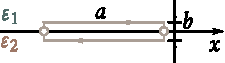
\includegraphics[scale=1.0]{figures/ch_02/fig_2_9.pdf}
			\caption[]{}
			\label{fig:2_9}
		\end{center}
	\end{minipage}
	\hfill{}%space{-0.05cm}
	\begin{minipage}[t]{0.48\linewidth}
		\begin{center}
			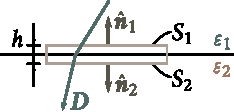
\includegraphics[scale=1.0]{figures/ch_02/fig_2_10.pdf}
			\caption[]{}
			\label{fig:2_10}
		\end{center}
	\end{minipage}
\vspace{-0.4cm}
\end{figure}

Substituting in accordance with \eqn{2_21} the projections of the vector $\vec{D}$ divided by $\varepsilon_0\varepsilon$ for the projections of the vector $\vec{E}$, we get the proportion
\begin{equation*}
    \frac{D_{1,\tau}}{\varepsilon_0\varepsilon_1} = \frac{D_{2,\tau}}{\varepsilon_0\varepsilon_2}
\end{equation*}

\noindent
whence it follows that
\begin{equation}\label{eq:2_45}
    \frac{D_{1,\tau}}{D_{2,\tau}} = \frac{\varepsilon_1}{\varepsilon_2}.
\end{equation}

Now let us take an imaginary cylindrical surface of height $h$ on the interface between the dielectrics (\fig{2_10}). Base $S_1$ is in the first dielectric, and base $S_2$ in the second. Both bases are identical in size ($S_1=S_2=S$) and are so small that within the limits of each of them the field may be considered homogeneous. Let us apply Gauss's theorem [see \eqn{2_25}] to this surface. If there are no extraneous charges on the interface between the dielectrics, the right-hand side in \eqn{2_25} equals zero. Hence, $\Phi_D=0$.

The flux through base $S_1$ is $D_{1,n}S$, where $D_{1,n}$ is the projection of the vector $\vec{D}$ in the first dielectric onto the normal $\hatvec{n}_1$. Similarly, the flux through base $S_2$ is $D_{2,n}S$, where $D_{2,n}$ is the projection of the vector $\vec{D}$ in the second dielectric onto the normal $\hatvec{n}_2$. The flux through
the side surface can be written in the form $\average{D}_n\ab{S}{side}$, where $\average{D}_n$ is the value of $D_n$ averaged over the entire side surface, and $\ab{S}{side}$ is the magnitude of this surface. We can thus write that
\begin{equation}\label{eq:2_46}
    \Phi_D = D_{1,n} S + D_{2,n} S + \average{D}_n\ab{S}{side} = 0.
\end{equation}

\noindent
If the altitude $h$ of the cylinder is made to tend to zero, then $\ab{S}{side}$ will also tend to zero. Hence, in the limit, we get
\begin{equation*}
    D_{1,n} = - D_{2,n}.
\end{equation*}

\noindent
Here $D_{i,n}$ is the projection onto $\hatvec{n}_i$ of the vector $\vec{D}$ the $i$-th dielectric in direct proximity to its interface with the other dielectric. The signs of the projections are different because the normals $\hatvec{n}_1$ and $\hatvec{n}_2$ to the bases of the cylinder have opposite directions. If we project $\vec{D}_1$ and $\vec{D}_2$ onto the same normal, we get the condition
\begin{equation}\label{eq:2_47}
    D_{1,n} = D_{2,n}.
\end{equation}

Using \eqn{2_21} to replace the projections of $\vec{D}$ with the corresponding projections of the vector $\vec{E}$ multiplied by $\varepsilon_0\varepsilon$, we get the relation
\begin{equation*}
    \varepsilon_0 \varepsilon_1 E_{1,n} = \varepsilon_0 \varepsilon_2 E_{2,n}
\end{equation*}

\noindent
whence
\begin{equation}\label{eq:2_48}
    \frac{E_{1,n}}{E_{2,n}} = \frac{\varepsilon_2}{\varepsilon_1}.
\end{equation}

The results we have obtained signify that when passing through the interface between two dielectrics, the normal component of the vector $\vec{D}$ and the tangential component of the vector $\vec{E}$ change continuously. The tangential component of the vector $\vec{D}$ and the normal
component of the vector $\vec{E}$, however, are disrupted when passing through the interface.

Equations \eqref{eq:2_44}, \eqref{eq:2_45}, \eqref{eq:2_47}, and \eqref{eq:2_48} determine the conditions which the vectors $\vec{E}$ and $\vec{D}$ must comply with on the interface between two dielectrics (if there are no extraneous charges on this interface). We have obtained these equations for an electrostatic field. They also hold, however, for fields varying with time (see
\sect{16_3}).

The conditions we have found also hold for the interface between a dielectric and a vacuum. In this case, one of the permittivities must be taken equal to unity.

We must note that condition \eqref{eq:2_47} can be obtained on the basis of the fact that the displacement lines pass through the interface between two dielectrics without being interrupted (\fig{2_11}). According
to the rule for drawing these lines, the number of lines arriving at area $\Delta{S}$ from the first dielectric is $D_1\Delta{S}_1=D_1\Delta{S}\cos\alpha_1$. Similarly, the number of lines emerging from area $\Delta{S}$ into the second dielectric is $D_2\Delta{S}_2=D_2\Delta{S}\cos\alpha_2$. If the lines are not interrupted at the interface, both these numbers must be the same:
\begin{equation*}
    D_1\Delta{S}\cos\alpha_1 = D_2\Delta{S}\cos\alpha_2.
\end{equation*}

\noindent
Cancelling $\Delta{S}$ and taking into account that the product $D\cos\alpha$ gives the value of the normal component of the vector $\vec{D}$, we arrive at condition \eqref{eq:2_47}.

The displacement lines are bent (refracted) on the interface between dielectrics, owing to which the angle $\alpha$ between a normal to the interface and the line $\vec{D}$ changes. Inspection of \fig{2_12} shows
that
\begin{equation*}
    \tan\alpha_1 : \tan\alpha_2 = \frac{D_{1,\tau}}{D_{1,n}} : \frac{D_{2,\tau}}{D_{2,n}}
\end{equation*}

\noindent
whence with account taken of Eqs. \eqref{eq:2_45} and \eqref{eq:2_47}, we get the law of displacement line refraction:
\begin{equation}\label{eq:2_49}
    \frac{\tan\alpha_1}{\tan\alpha_2} = \frac{\varepsilon_1}{\varepsilon_2}.
\end{equation}

\noindent
When displacement lines pass into a dielectric with a lower permittivity $\varepsilon$, the angle made by them with a normal diminishes, hence, the lines are spaced farther apart; when the lines pass into a dielectric with a higher permittivity $\varepsilon$, on the contrary, they become closer together.

\begin{figure}[t]
	\begin{minipage}[t]{0.48\linewidth}
		\begin{center}
			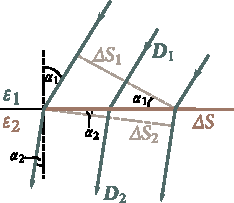
\includegraphics[scale=1.1]{figures/ch_02/fig_2_11.pdf}
			\caption[]{}
			\label{fig:2_11}
		\end{center}
	\end{minipage}
	\hfill{}%space{-0.05cm}
	\begin{minipage}[t]{0.48\linewidth}
		\begin{center}
			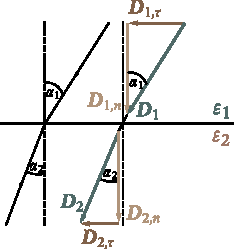
\includegraphics[scale=1.1]{figures/ch_02/fig_2_12.pdf}
			\caption[]{}
			\label{fig:2_12}
		\end{center}
	\end{minipage}
\vspace{-0.4cm}
\end{figure}

\section{Forces Acting on a Charge in a Dielectric}\label{sec:2_8}

If we introduce into an electric field in a vacuum a charged body of such small dimensions that the external field within the body can be considered homogeneous, then the body will experience the force
\begin{equation}\label{eq:2_50}
    \vec{F} = q \vec{E}.
\end{equation}

\noindent
To place a charged body in a field set up in a dielectric, a cavity must be made in the latter. In a fluid dielectric, the body itself forms the cavity by displacing the dielectric from the volume it occupies. The field inside the cavity $\ab{\vec{E}}{cav}$ will differ from that in a continuous dielectric. Thus, we cannot calculate the force exerted on a charged body placed in a cavity as the product of the charge $q$ and the field strength $\vec{E}$ in the dielectric before the body was introduced into it.

When calculating the force acting on a charged body in a fluid dielectric, we must take another circumstance into account. Mechanical tension is set up on the boundary with the body in the dielectric. This sets up an additional mechanical force $\ab{\vec{F}}{ten}$ acting on the body.

Thus, the force acting on a charged body in a dielectric, generally speaking, cannot be determined by \eqn{2_50}, and it is usually a very complicated task to calculate it. These calculations give an interesting result for a fluid dielectric. The resultant of the electric force $q\ab{\vec{E}}{cav}$ and the mechanical force $\ab{\vec{F}}{ten}$ is found to be exactly equal to $q\vec{E}$, where $\vec{E}$ is the field strength in the continuous dielectric
\begin{equation}\label{eq:2_51}
    \vec{F} = q\ab{\vec{E}}{cav} + \ab{\vec{F}}{ten} = q\vec{E}.
\end{equation}

The strength of the field produced in a homogeneous infinitely extending dielectric by a point charge is determined by \eqn{2_49}. Hence, we get the following expression for the forces of interaction of two point charges immersed in a homogeneous infinitely extending dielectric:
\begin{equation}\label{eq:2_52}
    F = \frac{1}{4\pi\varepsilon_0} \frac{q_1q_2}{\varepsilon r^2}.
\end{equation}

\noindent
This formula expresses Coulomb's law for charges in a dielectric. It holds only for fluid dielectrics.

Some authors characterize \eqn{2_52} as ``the most general expression of Coulomb's law''. In this connection, we shall cite Richard P. Feynman: ``Many older books on electricity start with the 'fundamental' law that the force between two charges is\ldots [\eqn{2_52} is given]\ldots, a point of view which is thoroughly unsatisfactory. For one thing, it is not true in general; it is true only for a world filled with a liquid. Secondly, it depends on the fact that $\varepsilon$ is a constant which is only approximately true for most real materials''\footnote{R. P. Feynman, R. B. Leighton, M. Sands. The Feynman Lectures on Physics. Vol. II. Reading, Mass., Addison-Wesley (1965), p. 10-8.}.

We shall not treat questions relating to the forces acting on a charge inside a cavity made in a solid dielectric.

\section{Ferroelectrics}\label{sec:2_9}

There is a group of substances that can have the property of spontaneous polarization in the absence of an external field. They are called \textbf{ferroelectrics}. This phenomenon was first discovered for Rochelle salt, and the first detailed investigation of the electrical properties of this salt was carried out by the Soviet physicists I. Kurchatov and P. Kobeko.

Ferroelectrics differ from the other dielectrics in a number of features:

1. Whereas the permittivity $\varepsilon$ of ordinary dielectrics is only several units, reaching as an exception several scores (for example, for water $\varepsilon=81$), the permittivity of ferroelectrics may be of the order of several thousands.

2. The dependence of $P$ on $E$ is not linear (see branch $1$ of the curve shown in \fig{2_13}). Hence, the permittivity depends on the field strength.

3. When the field changes, the values of the polarization $P$ (and, therefore, of the displacement $D$ too) lag behind the field strength $E$. As a result, $P$ and $D$ are determined not only by the value of $E$ at the given moment, but also by the preceding values of $E$, \ie, they depend on the preceding history of the dielectric. This phenomenon is called \textbf{hysteresis} (from the Greek word ``husterein''---to come late, be behind). Upon cyclic changes of the field, the dependence of $P$ on $E$ follows the curve shown in \fig{2_13} and called a \textbf{hysteresis loop}.
When the field is initially switched on, the polarization grows with $E$ according to branch $1$ of the curve. Diminishing of $P$ takes place along branch $2$. When $E$ vanishes, the substance retains a value of the polarization $\ab{P}{r}$ called the \textbf{residual polarization}. The polarization vanishes only under the action of an oppositely directed field $\ab{E}{c}$. This value of the field strength is called the \textbf{coercive force}. Upon a further change in $E$, branch $3$ of the hysteresis loop is obtained, and so on.

\begin{figure}[t]
    \begin{center}
		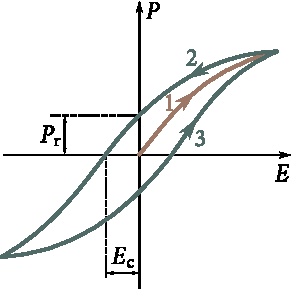
\includegraphics[scale=1.0]{figures/ch_02/fig_2_13.pdf}
		\caption[]{}
		\label{fig:2_13}
	\end{center}
    \vspace{-0.8cm}
\end{figure}

The behaviour of the polarization of ferroelectrics is similar to that of the magnetization of ferromagnetics (see \sect{7_9}), and this is the origin of their name.

Only crystalline substances having no centre of symmetry can be ferroelectrics. For example, the crystals of Rochelle salt belong to the rhombic system (see Sec. 13.2 of Vol. I). The interaction of the particles in a ferroelectric crystal leads to the fact that their dipole moments line up spontaneously parallel to one another. In exclusive cases, the identical orientation of the dipole moments extends to the entire crystal. Ordinarily, however, regions appear in a crystal in whose confines the dipole moments are parallel to one another, but the directions of polarization in different regions are different. Thus, the resultant moment of an entire crystal may equal zero. The regions of spontaneous polarization are also called \textbf{domains}. Under the action of an external field, the moments of the domains rotate as a single whole, arranging themselves in the direction of the field.

Every ferroelectric has a temperature at which the substance loses its unusual properties and becomes a normal dielectric. This temperature is called the \textbf{Curie point}. Rochelle salt has two Curie points, namely, \SI{-15}{\degreeCelsius} and \SI{+22}{\degreeCelsius}, and it behaves like a ferroelectric only in the interval between these two temperatures. Its electrical properties are conventional at temperatures below \SI{-15}{\degreeCelsius} and above \SI{+22}{\degreeCelsius}.
